\subsection{Упражнение 1}

«A Soft Murmur» — это веб-сайт, на котором можно послушать множество естественных источников шума, включая дождь, волны, ветер и т. д. 

\noindent На http://asoftmurmur.com/about/ вы можете найти их список записей, большинство из которых находится на http://freesound.org.

\noindent Загрузите несколько таких файлов и вычислите спектр каждого сигнала. Спектр мощности похож на белый шум, розовый шум, или броуновский шум? Как изменяется спектр во времени?

Возьмем звук моря и выделим два сегмента.

\begin{lstlisting}[language=Python]
if not os.path.exists('13793__soarer__north-sea.wav'):
    !wget https://drive.google.com/file/d/1OJcFGqEs128g5T8pQmgaERBHX8cyFSsT/view?usp=sharing
from thinkdsp import read_wave
wave = read_wave('13793__soarer__north-sea.wav')
wave.make_audio()
segment = wave.segment(start=15, duration=1.0)
segment.make_audio()
segment.plot()
\end{lstlisting}
\begin{figure}[H]
	\begin{center}
		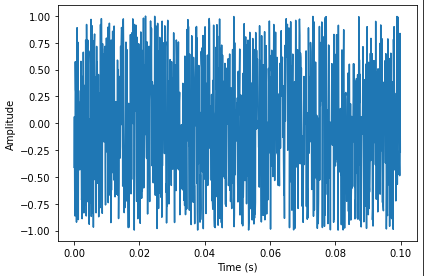
\includegraphics[scale=1]{fig/lab04/lab4_1.png}
		\caption{График сигнала}
	\end{center}
\end{figure}

Определим характеристики шума.

\begin{lstlisting}[language=Python]
from thinkdsp import decorate
spectrum.plot_power()

loglog = dict(xscale='log', yscale='log')
decorate(xlabel='Frequency (Hz)',
         ylabel='Power', 
         **loglog)
\end{lstlisting}
\begin{figure}[H]
	\begin{center}
		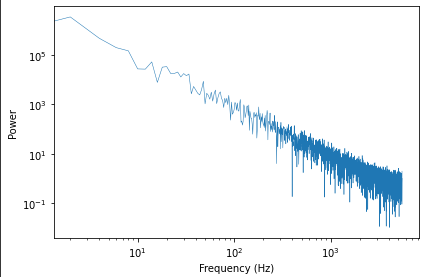
\includegraphics[scale=1]{fig/lab04/lab4_2.png}
		\caption{Спектр в логорифмическом масштабе}
	\end{center}
\end{figure}

График напоминает белый шум. Далее возьмем идущий за ним другой сегмент.

\begin{lstlisting}[language=Python]
segmentNext = wave.segment(start=16, duration=1.0)
segmentNext.make_audio()

spectrumNext = segmentNext.make_spectrum()
spectrum.plot_power()
spectrumNext.plot_power()

loglog = dict(xscale='log', yscale='log')
decorate(xlabel='Frequency (Hz)',
         ylabel='Power', 
         **loglog)
\end{lstlisting}
\begin{figure}[H]
	\begin{center}
		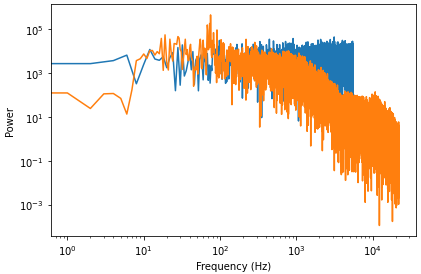
\includegraphics[scale=1]{fig/lab04/lab4_3.png}
		\caption{Сравнение спектров в логорифмическом масштабе}
	\end{center}
\end{figure}


\subsection{Упражнение 2}

Реализуйте метод Бартлетта\cite{barlett} и используйте его для оценки спектра мощности шумового сигнала. Подсказка: посмотрите на реализацую make\_spectrogram.

Реализуем метод Бартлетта для оценки спектра мощности шумового сигнала. Данный метод будет разделять сигнал на сегменты, вычислять для них разложение Фурье, вычислять сумму квадратов, находить среднее и вычислять корень.


\begin{lstlisting}[language=Python]
from thinkdsp import Spectrum

def make_barlett(wave, N, flag=True):
  spectrogram = wave.make_spectrogram(N,flag)
  spec_mac = spectrogram.spec_map.values()

  powers = []
  for spectrum in spec_mac:
    powers.append(spectrum.power)
  
  hs = np.sqrt(sum(powers)/ len(powers))
  fs = next(iter(spec_mac)).fs

  return Spectrum(hs, fs, wave.framerate)
\end{lstlisting}

Проведем тестирование на сигнале с предыдущего задания.

\begin{lstlisting}[language=Python]
barlett = make_barlett(segmentNext,1024)
barlett.plot_power()
decorate(xlabel='Frequency (Hz)', 
         ylabel='Power', 
         **loglog)
\end{lstlisting}

\begin{figure}[H]
	\begin{center}
		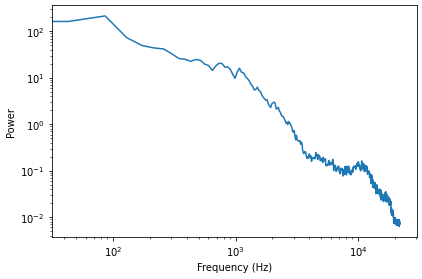
\includegraphics[scale=1]{fig/lab04/lab4_4.png}
		\caption{Результат работы функции}
	\end{center}
\end{figure}


\subsection{Упражнение 3}

Загрузите в виде CSV-файла исторические данные о ежедневной цене BitCoin. Откройте этот файл и вычислите спектр цен BitCoin как функцию времени. Похоже ли это на белый, розовый или броуновский шум?

Скачаем csv файл с ценами на биткоин.

\begin{lstlisting}[language=Python]
if not os.path.exists('market-price.csv'):
    !wget https://github.com/pimenov01/telecom/raw/main/files/market-price.csv
import csv
worth = []
with open('market-price.csv') as File:
  reader = csv.reader(File, delimiter=',', quotechar=',',
                        quoting=csv.QUOTE_MINIMAL)
  for row in reader:
    worth.append(row[1])
worth = worth [1:]
days = a=np.arange(0,len(worth))
\end{lstlisting}
\begin{lstlisting}[language=Python]
from thinkdsp import Wave
wave = Wave(worth,days,1)
spectrum = wave.make_spectrum()
spectrum.plot_power()
decorate(xlabel='Частота',
         ylabel='Мощность', 
         **loglog)
\end{lstlisting}

\begin{figure}[H]
	\begin{center}
		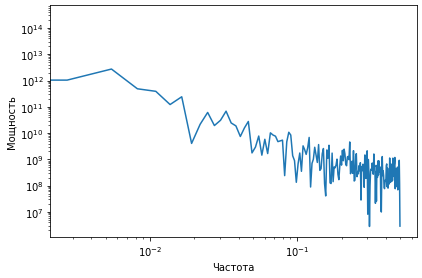
\includegraphics[scale=1]{fig/lab04/lab4_5.png}
		\caption{Спектрограмма цен BitCoin в логорифмическом формате}
	\end{center}
\end{figure}

Больше всего напоминает красный шум.

\subsection{Упражнение 4}

Счетчик Гейгера — это прибор, который регистрирует радиацию. Когда ионизирующая частица попадает на детектор, он генерирует всплеск тока. Общий вывод в определенный момент времени можно смоделировать как некоррелированный шум Пуассона (UP), где каждая выборка представляет собой случайную величину из распределения Пуассона, которая соответствует количеству частиц, обнаруженных в течение интервала.

Напишите класс с именем `UncorrelatedPoissonNoise`, который наследуется от `\_Noise` и предоставляет `evaluate`. Он должен использовать `np.random.poisson` для генерации случайных значений из распределения Пуассона. Параметр этой функции, lam, представляет собой среднее число частиц в течение каждого интервала. Вы можете использовать атрибут `amp`, чтобы указать `lam`. Например, если частота кадров равна 10 кГц, а amp равно 0,001, мы ожидаем около 10 «кликов» в секунду.

Создайте около секунды шума UP и послушайте его. Для низких значений «ампер», например 0,001, это должно звучать как счетчик Гейгера. Для более высоких значений это должно звучать как белый шум. Вычислите и начертите спектр мощности, чтобы увидеть, похож ли он на белый шум.

Напишем класс UncorrelatedPoissonNoise, который наследуется от класса thinkdsp\_Noise и который моделирует некоррелированный пуассонвский шум (UP).

\begin{lstlisting}[language=Python]
from thinkdsp import *
class UncorrelatedPoissonNoise(Noise):
    def evaluate(self, ts):
        ys = np.random.poisson(self.amp, len(ts))
        return ys
\end{lstlisting}
Сгенирируем сигнал с маленькой амплитудой, звук должен быть похож на счетчик Гейгера.
\begin{lstlisting}[language=Python]
firstSignal = UncorrelatedPoissonNoise(amp=0.001)
firstWave = firstSignal.make_wave(duration=1, framerate=10000)
firstWave.make_audio()
\end{lstlisting}

Далее сгенерируем сигнал с большой амплитудой.

\begin{lstlisting}[language=Python]
secondSignal = UncorrelatedPoissonNoise(1)
secondWave = secondSignal.make_wave(duration=1,framerate = 10000)
secondWave.make_audio()
\end{lstlisting}

Посмотрим на характеристики данных сигналов:

\begin{lstlisting}[language=Python]
spectrum1 = firstWave.make_spectrum()
spectrum2 = secondWave.make_spectrum()

spectrum1.plot_power()
spectrum2.plot_power()

decorate(xlabel='Частота', 
         ylabel='Мощность', 
         **loglog)
\end{lstlisting}
\begin{figure}[H]
	\begin{center}
		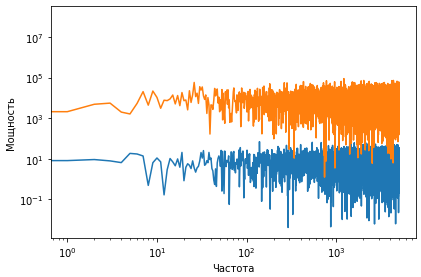
\includegraphics[scale=1]{fig/lab04/lab4_6.png}
		\caption{Сравнение спектров}
	\end{center}
\end{figure}

Видно, что при увеличении амплитуды звук больше похож на белый шум.

\subsection{Упражнение 5}

В этой главе описан алгоритм генерации розового шума. Концептуально простой, но вычислительно затратный. Есть более эффективные альтернативы, такие как алгоритм Восса-Маккартни.

Используем алгоритм Voss-McCartney для генерации розового шума.

\begin{lstlisting}[language=Python]
def voss(nrows, ncols=16):
    array = np.empty((nrows, ncols))
    array.fill(np.nan)
    array[0, :] = np.random.random(ncols)
    array[:, 0] = np.random.random(nrows)
    
    n = nrows
    cols = np.random.geometric(0.5, n)
    cols[cols >= ncols] = 0
    rows = np.random.randint(nrows, size=n)
    array[rows, cols] = np.random.random(n)

    df = pd.DataFrame(array)
    df.fillna(method='ffill', axis=0, inplace=True)
    total = df.sum(axis=1)

    return total.values
\end{lstlisting}

\begin{lstlisting}[language=Python]
ys = voss(11025,16)
wave = Wave(ys)
wave.plot()
\end{lstlisting}

\begin{figure}[H]
	\begin{center}
		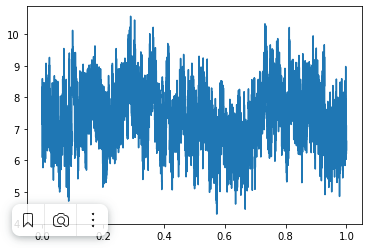
\includegraphics[scale=1]{fig/lab04/lab4_7.png}
		\caption{Сгенерированный сигнал}
	\end{center}
\end{figure}

\begin{lstlisting}[language=Python]
spectrum = wave.make_spectrum()
spectrum.hs[0] = 0
spectrum.plot_power()
decorate(xlabel='Частота',
         ylabel='Мощность',
         **loglog)
\end{lstlisting}
\begin{figure}[H]
	\begin{center}
		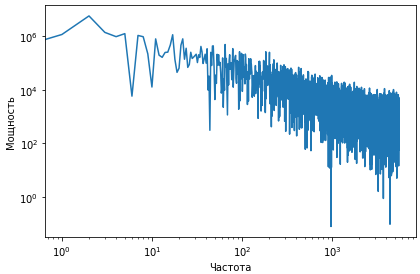
\includegraphics[scale=1]{fig/lab04/lab4_8.png}
		\caption{Спектр сигнала}
	\end{center}
\end{figure}

\begin{lstlisting}[language=Python]
spectrum.estimate_slope()[0]
\end{lstlisting}

-0.9809177359665783

\noindent Видим, что в итоге был получен сигнал розового шума.

\subsection{Вывод}

В ходе данной ЛР были изучены различные виды шумов: белый, розовый, красный и т. д. Шум - это сишнал, представленный компонентами с разными частотами, но не имеющий гармонической структура периодических сигналов.
